\chapter{Inleiding}
\label{ch:inleiding}

%De inleiding moet de lezer net genoeg informatie verschaffen om het onderwerp te begrijpen en in te zien waarom de onderzoeksvraag de moeite waard is om te onderzoeken. In de inleiding ga je literatuurverwijzingen beperken, zodat de tekst vlot leesbaar blijft. Je kan de inleiding verder onderverdelen in secties als dit de tekst verduidelijkt. Zaken die aan bod kunnen komen in de inleiding~\autocite{Pollefliet2011}:


%\begin{itemize}
 % \item context, achtergrond
  %\item afbakenen van het onderwerp
  %\item verantwoording van het onderwerp, methodologie
  %\item probleemstelling
  %\item onderzoeksdoelstelling
  %\item onderzoeksvraag
  %\item \ldots
%\end{itemize}

 De ontwikkeling van mobiele applicaties is een belangrijke niche in de IT. Zo kunnen we drie verschillende besturingssystemen onderscheiden bij mobiele applicaties: Android, iOS en Windows. Die laatste wordt steeds minder en minder gebruikt voor mobiele toepassingen. Volgens het artikel \textcite{Statista2018}, van Statista, een portaal voor statistieken en onderzoek, heeft Android een marktaandeel van 87.7\% wereldwijd. Dit wil dus zeggen dat meer dan 85\% van de mensen die een smartphone heeft, een toestel heeft met het Android besturingssysteem. 

 De mobiele applicaties die draaien op Android werden allemaal geprogrammeerd in Java. Maar sinds kort is er een nieuwe mogelijkheid, Kotlin. Kotlin is een programmeertaal die ontworpen is door JetBrains in 2011. Zes jaar later (2017) biedt Google volledige ondersteuning om Android-applicaties te programmeren in Kotlin. Kotlin zou initieel ontwikkeld zijn om de productiviteit van JetBrains te vergroten. Zie sectie \ref{sec:whykotlin} voor meer uitleg.
 
 \section{Begrippen}
 \subsection{Wat is cross-platform?}
 Wat is de betekenis van cross-platform? Gaat dit over het delen van user interfaces, het delen van domeinlogica, of gaat dit over beiden? \textcite{CrossExplain}, een website voor IT professionals en geeks, heeft op hun website een verklaring voor een cross-platform product. Zij verklaren dat een cross-platform product een platformonafhankelijk computerproduct of systeem is dat op meerdere platformen of besturingssystemen kan werken. Zij geven echter ook aan dat wanneer bepaalde zaak van de applicatie hergebruikt worden per platform, er gedaan wordt aan cross-platform development. Zowel het delen van domeinlogica, het delen van interfaces of beiden is cross-platform ontwikkeling. Cross-platform is echter ook bekend als multiplatform of platformonafhankelijk.
 
\subsection{Wat is een framework?}
Een framework kan in het algemeen beschreven worden als een soort van structuur die bedoeld is als ondersteuning bij het bouwen van een bepaald iets. Het is goed te vergelijken met een skelet waarop iets wordt gebouwd en het biedt functionaliteiten aan om te focussen op bepaalde specifieke taken. 

Frameworks worden sterk gebruikt bij het ontwikkelen van software en vooral in de wereld van de mobiele applicaties. Momenteel bestaan er verschillende frameworks waarmee mobiele applicaties kunnen worden gebouwd. Twee voorbeelden hiervan zijn Cordova en PhoneGap \autocite{Framework}.

\subsection{Wat is een native applicatie?}
Een native applicatie is een softwareprogramma dat ontwikkeld is om gebruik te worden op een specifiek platform of besturingssysteem. Aangezien een native applicatie gebouwd is om op een bepaalde platform te worden gebruikt, kan het gebruik maken van de hardware en software van het toestel. Native applicaties kunnen geoptimaliseerde prestaties bieden en hebben het voordeel om gebruik te kunnen maken van de laatst nieuwe technologieën zoals GPS, wat veel moeilijker is bij bijvoorbeeld een webapplicatie \autocite{MeaningNativeApp}.

\subsection{Wat is een hybride applicatie?}
Een hybride applicatie is een applicatie die de features van enerzijds een native applicatie en anderzijds een webapplicatie combineert. Hybride applicaties worden dus niet ontwikkeld met de bedoeling om gebruik te worden op een bepaald platform of besturingssysteem. De bedoeling van hybride applicaties is om de mogelijk aan te bieden om de applicatie op eender welk besturingssysteem te gebruiken. Hybride applicaties maken gebruik van een ingebouwde browser om de user interface te weer te geven. Bij hybride applicatieontwikkeling wordt er gebruik gemaakt van Javascript, HTML en CSS. Enkele voorbeelden van dit type framework zijn Cordova, Ionic en Trigger.IO \autocite{MeaningHybridApp}.

\subsection{Wat is een cross-platform applicatie?}
Cross-platform applicaties zijn gelijkaardig aan hybride applicaties. Het grote verschil tussen beide types is dat cross-platform applicaties geen gebruik maken van een ingebouwde browser om de user interface te tonen aan de gebruiker. De user interface wordt getoond aan de hand van native elementen. Javascript wordt gebruikt om de functionaliteiten in de applicatie op te bouwen. HTML en CSS zorgen voor de opbouw van de user interface. Enkele voorbeelden van dit type framework zijn Xamarin, React/Native en NativeScript \autocite{NativeVsCross2}.

\subsection{Native versus cross-platform- en hybride development}
\label{sec:nativeversuscross}
Voor het ontwikkelen van mobiele applicaties bestaan er dus verschillende methodes. Het wel of niet kiezen voor native applicatieontwikkeling is afhankelijk van heel wat criteria. Denk maar aan de platformen dat de applicatie moet ondersteunen, de eisen waaraan een applicatie moet voldoen, de verschillende functionaliteiten en ga zo maar door. Iedere methodiek voor het ontwikkelen van applicaties heeft zo zijn eigen voor- en nadelen (\textcite{NativeVsCross2}, \textcite{NativeVsCross3}).

\subsubsection{Native ontwikkeling}
Voordelen:
\begin{itemize}
	\item Groot aantal functionaliteiten aangezien er gebruik kan worden gemaakt van alle mogelijkheden van het gebruikte toestel.
	\item Snelle software prestaties.
	\item Een user interface die overeenkomt met de gebruikerservaringen van het besturingssysteem.
\end{itemize}

Nadelen:
\begin{itemize}
	\item Indien er meerdere platformen ondersteund moeten worden, moeten er twee aparte applicaties ontwikkeld worden.
	\item Kosten om meerdere platformen te beheren.
	\item Er kan geen code gedeeld worden tussen verschillende platformen.
\end{itemize}

\subsubsection{Cross-platform- en hybride ontwikkeling}
Voordelen:
\begin{itemize}
	\item Applicatie kan sneller ontwikkeld worden.
	\item Verschillende frameworks die helpen bij de ontwikkeling.
	\item Het delen van code over de verschillende platformen.
\end{itemize}

Nadelen:
\begin{itemize}
	\item Niet alle code kan gedeeld worden over de verschillende platformen. Soms moet er native code geschreven worden.
	\item Toegang tot het toestel en besturingssysteem zijn afhankelijk van de mogelijkheden van het framework.
	\item Snelheid van de applicatie kan trager zijn dan native applicatie aangezien er gewerkt wordt via een tussenliggende taal, namelijk Javascript.
	\item Vaak afhankelijk van third parties.
\end{itemize}

\section{Probleemstelling}
\label{sec:probleemstelling}
Vanuit dit onderzoek zal blijken hoe goed Kotlin/Native is als cross-platform framework en wat de mogelijkheden zijn van Kotlin/Native om een applicatie te programmeren voor verschillende platformen. Deze vraag kwam vanuit het bedrijf genaamd Endare BVBA. Endare is een bedrijf dat gericht is op het ontwikkelen van mobiele- en webapplicaties. Een developer bij Endare is reeds bezig met het aanleren van Kotlin en heeft reeds enkele Android-projecten gemaakt met Kotlin. Bij Endare wordt er zeer veel aan cross-platform ontwikkeling gedaan. Zo heeft een stagiair tijdens zijn stage bij Endare, gewerkt met React/Native, het populaire framework van Facebook voor cross-platform ontwikkeling.

De vraag naar native applicaties wordt steeds minder. Waarom? Uit sectie \ref{sec:nativeversuscross} bleek dat native applicaties voor veel bedrijven een grote kost zijn. Er is enerzijds twee keer (indien er voor iOS en Android ontwikkeld wordt) een kost om de applicaties te bouwen, anderzijds is er twee keer een kost om de applicaties te onderhouden of eventueel uit te breiden. Volgens een artikel van Comentum, een toonaangevend bedrijf op het gebied van digitale oplossingen, varieert de kost voor het ontwikkelen van een native applicatie (Android of iOS) tussen de 9000 en 90000 dollar, afhankelijk van de vereisten van de applicatie \autocite{NativeDevelopmentCost}. 

\begin{figure} [ht]
	\centering
	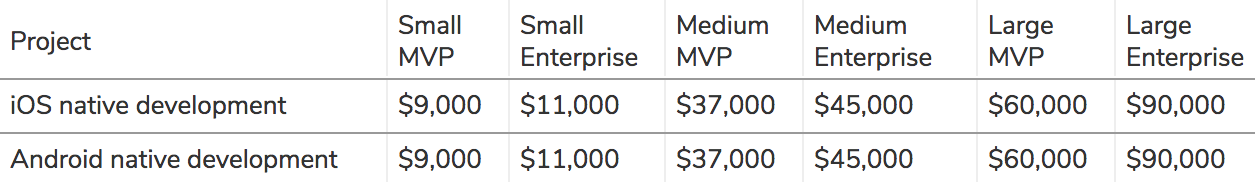
\includegraphics[width=0.95\textwidth]{img/nativeappkost.png}
	\caption{Kostprijs ontwikkeling native applicatie (\cite{NativeDevelopmentCost})}
	\label{fig:nativeappkost}
\end{figure}

Uit sectie \ref{sec:nativeversuscross} valt te besluiten dat er ook redenen zijn waarom bedrijven nu net wel native applicaties willen in plaats van cross-platform applicaties. 

Momenteel is er meer dan genoeg keuze om applicaties voor verschillende platformen tegelijkertijd te ontwikkelen. Met Kotlin/Native komt er een nieuw framework zich aanbieden. Dit framework is nog zeer jong en er bestaat bijna geen documentatie. Ontwikkelaars die dit framework willen gebruiken moeten momenteel zelf de werking van Kotlin/Native proberen achterhalen. Daarom is het belangrijk om te bestuderen of Kotlin een mogelijkheid biedt tot een nieuwe cross-platform programmeertaal, hoe de compiler van Kotlin ervoor kan zorgen dat het op meerdere platformen kan draaien en hoe men nu juist gebruik kan maken van Kotlin/Native. 

Voor Endare heeft deze bachelorproef een grote meerwaarde aangezien zij iedere dag met cross-platform frameworks aan de slag moeten. Kotlin/Native zou de mogelijkheid geven om native applicaties te ontwikkelen in combinatie met een domeinlogica die gedeeld wordt tussen de verschillende platformen.

%Uit je probleemstelling moet duidelijk zijn dat je onderzoek een meerwaarde heeft voor een concrete doelgroep. De doelgroep moet goed gedefinieerd en afgelijnd zijn. Doelgroepen als ``bedrijven,'' ``KMO's,'' systeembeheerders, enz.~zijn nog te vaag. Als je een lijstje kan maken van de personen/organisaties die een meerwaarde zullen vinden in deze bachelorproef (dit is eigenlijk je steekproefkader), dan is dat een indicatie dat de doelgroep goed gedefinieerd is. Dit kan een enkel bedrijf zijn of zelfs één persoon (je co-promotor/opdrachtgever).

\section{Onderzoeksvraag}
\label{sec:onderzoeksvraag}
De onderzoeksvragen voor deze bachelorproef zijn: 
\begin{itemize}
	\item Hoe zorgt de Kotlin compiler ervoor dat Kotlin op verschillende platformen kan gebruikt worden?
	\item Wat is de werking van Kotlin/Native?
	\item In hoeverre kan Kotlin gebruikt worden voor cross-platform applicatieontwikkeling?
\end{itemize}
%Wees zo concreet mogelijk bij het formuleren van je onderzoeksvraag. Een onderzoeksvraag is trouwens iets waar nog niemand op dit moment een antwoord heeft (voor zover je kan nagaan). Het opzoeken van bestaande informatie (bv. ``welke tools bestaan er voor deze toepassing?'') is dus geen onderzoeksvraag. Je kan de onderzoeksvraag verder specifiëren in deelvragen. Bv.~als je onderzoek gaat over performantiemetingen, dan 

\section{Onderzoeksdoelstelling}
\label{sec:onderzoeksdoelstelling}
Voor deze bachelorproef zijn er verschillende criteria van succes:
\begin{itemize}
	\item De werking van de compiler, die Kotlin gebruikt, documenteren
	\item Goede documentatie opstellen over de werking van Kotlin/Native
	\item Bepalen in hoeverre Kotlin gebruikt kan worden als cross-platform programmeertaal
\end{itemize}
%Wat is het beoogde resultaat van je bachelorproef? Wat zijn de criteria voor succes? Beschrijf die zo concreet mogelijk.

\section{Opzet van deze bachelorproef}
\label{sec:opzet-bachelorproef}
% Het is gebruikelijk aan het einde van de inleiding een overzicht te
% geven van de opbouw van de rest van de tekst. Deze sectie bevat al een aanzet
% die je kan aanvullen/aanpassen in functie van je eigen tekst.

De rest van deze bachelorproef is als volgt opgebouwd:

In Hoofdstuk~\ref{ch:stand-van-zaken} wordt een overzicht gegeven van de stand van zaken binnen het onderzoeksdomein, op basis van een literatuurstudie.

In Hoofdstuk~\ref{ch:methodologie} wordt de methodologie toegelicht en worden de gebruikte onderzoekstechnieken besproken om een antwoord te kunnen formuleren op de onderzoeksvragen.

In Hoofdstuk~\ref{ch:compiler} zal onderzocht worden, via een literatuurstudie, wat de werking is van de Kotlin compiler. Hoe ervoor kan gezorgd worden dat Kotlin ook op apparaten zonder een JVM kan draaien.

In Hoofdstuk~\ref{ch:kotlinnative} zal Kotlin/Native bestudeerd worden. Hierin zal de werking van Kotlin/Native gedocumenteerd worden.

In Hoofdstuk~\ref{ch:praktisch} zal er praktisch een Kotlin/Native project worden uitgewerkt.

In Hoofdstuk~\ref{ch:conclusie}, tenslotte, wordt de conclusie gegeven en een antwoord geformuleerd op de onderzoeksvragen. Daarbij wordt ook een aanzet gegeven voor toekomstig onderzoek binnen dit domein.

